\documentclass[12pt,a4paper]{article}
\usepackage[left=2cm, right=2cm, top=2cm, bottom=2cm]{geometry} % page setup
\usepackage[ngerman]{babel} % use german language e.g. for references
%\usepackage{fancyhdr} % extensive control of page headers and footers
\usepackage{parskip} % space in between paragraphs
%\usepackage{titlesec} % select alternative section titles

%\usepackage[autostyle, german=quotes]{csquotes} % better citations with citep
%\usepackage[sort&compress,round,comma]{natbib} % needed by csquotes
%\usepackage[colorlinks=true,urlcolor=blue,linkcolor=blue,citecolor=blue]{hyperref} % clickable references
\usepackage{enumitem} % control layout of itemize, enumerate, description
%\usepackage{siunitx} % units and numbers formatting

\usepackage{graphicx} % Required for inserting images
%\usepackage{subcaption} % subfigure with nice caption formats
%\usepackage{wrapfig} % wrapfigure inside of text
%\usepackage{float} % improved interface for floating objects (provides the [H] modifier)
%\usepackage[section]{placeins} % Allows \FloatBarrier, to prevent floats from beeing shown at the bottom of the document
%\usepackage{multirow} % table with multirows

%\usepackage{bm} % bold math
%\usepackage{amsfonts,amsmath,amssymb} % all the math stuff
\usepackage[T1]{fontenc} % better font encoding (ö, copypaste from pdf)
%\usepackage[utf8]{inputenc} % works with matplotlib
%\usepackage{lmodern} % works with matplotlib
%\usepackage{textcomp} % support for the Text Companion fonts, which provide many text symbols (such as baht, bullet, copyright, musicalnote, onequarter, section, and yen)
%\usepackage{mathtools} % for beautiful math
%\usepackage{mathabx} % \corresponds symbol
\usepackage{titling} % This package allows customization of the title and author
\usepackage{setspace}
\usepackage{blindtext}

%\pagestyle{fancy} % header and footer
%\fancyhf{} % only one name per header
%\fancyhead[L]{\leftmark} % header on the left
%\fancyfoot[C]{\thepage}

%\renewcommand*\labelenumi{[\theenumi]}

\setlength{\droptitle}{-60pt} % Adjust the vertical space between the title and the top of the page

\begin{document}
	Marvin Henke
	\begin{center}
		\LARGE \textbf{Lense-Thirring-Effekt}
	\end{center}
	
	\begin{figure}[ht]
		\centering
		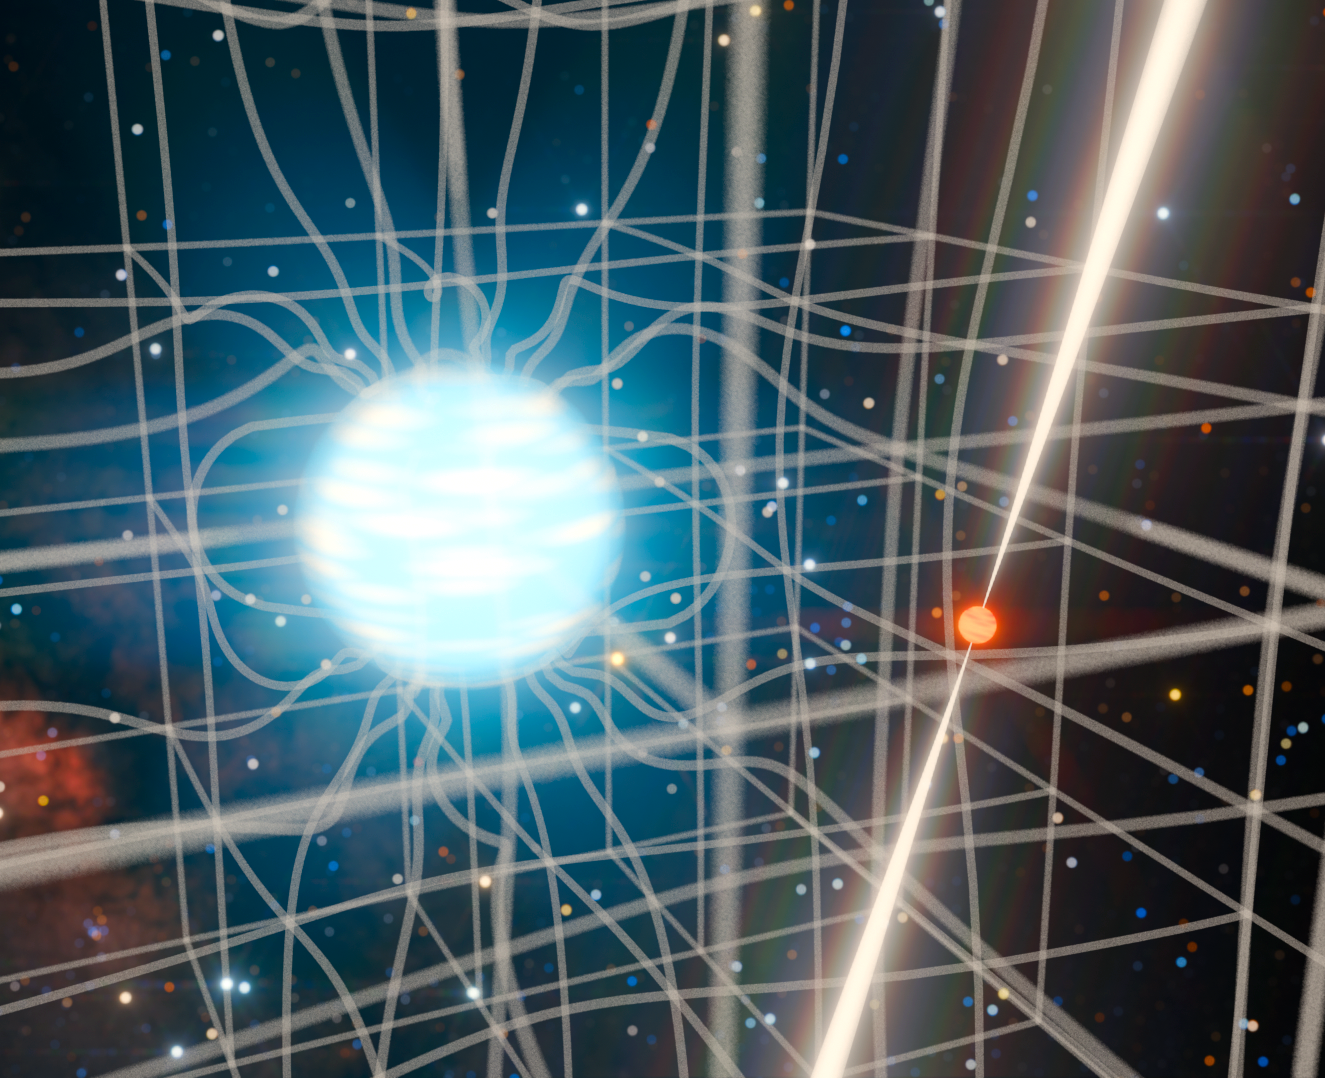
\includegraphics[width=0.75\textwidth]{../lense_thirring_edited.png}
	\end{figure}
	
	\noindent
	Nach Einstein wird die Raumzeit durch Masse gekrümmt. Rotiert die Masse sehr schnell, wird die Raumzeit wie zähflüssig mitbewegt. Der hierdurch erzeugte sogenannte Lense-Thirring (LT) Effekt wurde vor mehr als hundert Jahren im Rahmen der Allgemeinen Relativitätstheorie vorhergesagt, aber erst in den letzten Jahren gelang die experimentelle Beobachtung mit zufriedenstellender Genauigkeit [1].
	
	2020 wurde der LT-Effekt in einem einzigartigen Binärsystem aus Pulsar und schnell rotierendem weißen Zwerg beobachtet. Der LT-Effekt sorgt für eine Präzession des Orbits, was sich anhand der Strahlung des Pulsars messen lässt [3].
	Letztes Jahr wurde die LT-Präzession der Akkretionsscheibe eines supermassereichen Schwarzen
	Lochs beobachtet, die kurz nach dem Zerreißen eines Sterns entstanden ist [4].
	
	Wie hängt das alles mit Maxwellscher Elektrodynamik zusammen und lässt sich der LT-Effekt auch auf der Erde beobachten? Diese Fragen sowie die Theorie hinter den Beobachtungen werden in diesem Vortrag erklärt.
	
	\section*{Literatur}
	\begin{enumerate}[label={[\arabic*]}]
		\item J. Lense, H. Thirring, \textit{Phys. Z.} \textbf{19}, 156 (1918)
		\item C. Misner, K. Thorne, \& J. Wheeler. - Gravitation (1973)
		\item V. Venkatraman Krishnan \textit{et al.} Lense–Thirring frame dragging induced by a fast-rotating white dwarf in a binary pulsar system. \textit{Science} \textbf{367}, 577-580 (2020)
		\item D.R. Pasham, M. Zajaček, C.J. Nixon \textit{et al.} Lense–Thirring precession after a supermassive black hole disrupts a star. \textit{Nature} \textbf{630}, 325–328 (2024)
	\end{enumerate}
	
	\thispagestyle{empty}
	
\end{document}
